\documentclass[
	ngerman,
	fontsize=10pt,
	parskip=half,
	titlepage=true,
	DIV=12
]{scrartcl}

\usepackage[utf8x]{inputenc}
\usepackage{babel}
\usepackage[T1]	{fontenc}
\usepackage{lmodern}
\usepackage{microtype}
\usepackage{color}
\usepackage{csquotes}
\usepackage{amsmath}
\usepackage{hyperref}

\usepackage{minted}
	\usemintedstyle{xcode}

\usepackage{wrapfig}
\usepackage{graphicx}
\usepackage[bf]{caption} 
	\captionsetup{format=plain}

\usepackage{minted}
	\usemintedstyle{xcode}

\usepackage{tikz}
	\usetikzlibrary{calc}
	\usetikzlibrary{positioning}
	
\begin{document}

\part*{C-Kurs, Blatt 05, WiSe 2020}

\section{Kreuz- und Skalarprodukt mit structs (1P)}
Legen Sie eine \texttt{struct vector3d\_t} an, die eine $x$-, $y$- und eine $z$-Komponente umfasst. Überlegen Sie dazu zuerst, von welchem Datentyp die Records der \texttt{struct} sein müssen.

Erstellen Sie zwei Instanzen (zwei Variablen) vom Typ \texttt{struct vector3d\_t}, und speichern Sie darin zwei Vektoren (also jeweils drei Zahlenwerte).

Schreiben Sie nun je eine Funktion, die das Skalarprodukt und das Kreuzprodukt zweier Vektoren berechnet.
Welche Rückgabetypen müssen die beiden Funktionen haben?

\emph{Zur Erinnerung}:\\
Das Skalaprodukt zweier Vektoren ist folgendermaßen definiert:
\[ \vec{a} \cdot \vec{b} = a_x b_x + a_y b_y + a_z b_z \]
und das Kreuzprodukt erhalten Sie folgendermaßen:
\[
	\vec{a} \times \vec{b} =
	\begin{pmatrix}
		a_y b_z - a_z b_y\\
		a_z b_x - a_x b_z\\
		a_x b_y - a_y b_x
	\end{pmatrix}
\]

\emph{Tipp:} Für diese Aufgabe brauchen Sie \emph{keine} Pointer.

\emph{Lernziel: Structs, Funktionen}


\section{Karteisystem (2P)}
Legen Sie eine \texttt{struct person\_t} an, die Name, Alter und Körpergröße einer Person speichern kann. Erstellen Sie ein Array \texttt{people[3]}.

Schreiben Sie eine erste Funktion \texttt{enterPerson(struct person\_t * array, int ID)}, die das Array mittels \texttt{scanf} befüllt. Wozu braucht man die \texttt{int}-Variable?

Schreiben Sie anschließend eine zweite Funktion, die die Daten als Tabelle auf dem Bildschirm ausgibt.

\emph{Lernziel: \texttt{struct}s, Arrays, Schleifen}

\section{Matrixprodukt (3P)}
Bilden Sie Matrizen im Speicher mit folgendem \mintinline{c}{struct} ab:
\begin{minted}[linenos]{c}
typedef struct {
   int      rows;
   int      cols;
   double * data;
} matrix;
\end{minted}

Programmieren Sie dann das Matrixprodukt als Funktion. Es ist definiert als:
\[ c_{ij} = \sum_k a_{ik} \cdot b_{kj} \]

Ihre Funktion sollte folgenden Signatur haben:
\mint{c}{matrix MatProduct(matrix A, matrix B);}

Vergessen Sie nicht, reservierten Speicher wieder freizugeben.

Sie können auch eine Funktion schreiben, die die Matrix auf dem Bildschirm ausgibt:
\mint{c}{void MatPrint(matrix M);}

\emph{Lernziel: Dynamische Arrays, Schleifen}

Hier ein Beispiel:

\begin{gather*}
\begin{pmatrix}
1& 2\\
3& 4\\
5& 6\\
7& 8\\
\end{pmatrix}
\cdot
\begin{pmatrix}
3& 2& 1\\
5& 6& 7\\
\end{pmatrix}
=
\begin{pmatrix}
13& 14& 15\\
29& 30& 31\\
45& 46& 47\\
61& 62& 63\\
\end{pmatrix}
\end{gather*}

{\em Lernziel: Automatische Arrays, Schleifen}

\section{Optional: $\pi$ nach Monte-Carlo-Methode (1P)}
\begin{wrapfigure}{r}{.25\linewidth}
\vspace{-20pt}
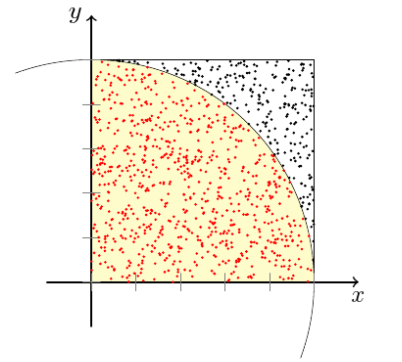
\includegraphics[width=\linewidth]{MCarlo}
\caption{\url{https://commons.wikimedia.org/wiki/File:Pi_statistisch.png}}
\vspace{-20pt}
\end{wrapfigure}
%
Schreiben Sie eine Funktion, die den Wert von $\pi$ näherungsweise berechnet. Gehen Sie dazu wie folgt vor:
\begin{itemize}
\item Generieren Sie \texttt{N} Paare von positiven Zufallszahlen $x, y$ zwischen 0 und 1
\item Berechnen Sie für jedes Wertepaar den Wert $x^2 + y^2$
\item Für jedes Wertepaar $(x, y)$, für das diese Summe kleiner oder gleich 1 ist, erhöhen Sie einen
	Zähler \texttt{counter}.
\item Der Wert \texttt{counter / N} nähert sich für große Werte von \texttt{N} dem Wert $\frac{\pi}{4}$
	an.
\end{itemize}

Schreiben Sie die Funktion so, dass ihr ein \emph{Genauigkeits-Parameter} übergeben wird. Dieser Parameter soll festlegen, wie viele Wertepaare $(x, y)$ erzeugt werden.

Zum Hintergrund:\newline
Für alle Punkte auf einem Kreis mit Mittelpunkt $(0,0)$ und Radius $R$ gilt:
\[ x^2 + y^2 = R^2\]
Das oben beschriebene Verfahren zählt also alle Punkte, die \emph{innerhalb} des Kreises oder auf der Kreislinie liegen. Die Anzahl der Punkte innerhalb des Kreises ist ein Maß für seine Fläche. Wie Sie wissen, gilt für die Fläche $A$ eines Kreises:
\[ A = R^2 \cdot \pi \]
Da wir nur positive Werte für $(x, y)$ betrachten, erhalten wir auch nur die Fläche eines \emph{Viertelkreises}. Indem wir $R=1$ setzen, sparen wir uns die Division durch $R^2$.

\emph{Lernziel: Schleifen, Funktionen}

\end{document}
